
With the increasingly large volumes of data, there is an urgent need to provide expressive and efficient data analytic tools. Datalog, a declarative logical programming language, has been widely implemented  due to its superiority of concise expressing and efficient execution of recursive queries. In this chapter, we focus on extending the expressive power of the language in the data scientists' familiar ways. We propose the LLib,  Logical Libraries, to provide a wide range of Datalog algorithms on top of BigDatalog and Apache Spark.  LLib encapsulates all the complex logic of algorithms into high-level APIs to simplify the development and   provides a unified interface similar to the Spark MLlib. LLib is proposed to be  DataFrame-based so that it can flexibly collaborate with other existing Spark operations in MLlib, Spark SQL, etc.
Considering the requirements for developing novel recursive applications not contained in LLib, we also show a new LFrame-based Datalog programming interface. The LFrame is an extension to the Spark DataFrame data structure and works in the similar way. Except the normal relational operations like projection, selection, the LFrame could support  logical operations like definitions of recursive rules and base relations. To visually show the expressive power of LLib and LFrame, we utilize amounts of running examples during description. 

\section{Introduction}
In the era of big data, the demand for flexible analytics of large-scale data has driven the researchers to build various general-purpose user-friendly platforms like Apache Spark   \citep{zaharia2012resilient}, AsterixDB \citep{alsubaiee2014asterixdb}, Pig \citep{olston2008pig}, Hive \citep{thusoo2009hive}, etc.  Among these systems, Spark is getting more and more attractive due to its efficient in-memory computation and abundant APIs (i.e. Spark SQL, GraphX, MLlib and SparkR) for complex analytics  to extract the rich information encapsulated in the data.

However, for the iterative applications like identifying the transitive closures or connected components of millions of vertexes, there are no dedicated designs for optimization among recursions in Spark because each iteration is contained in an identical job.  For the more advanced recursive analytics, the programming needs deep understanding and extensive knowledge of the platform.  To solve these issues, the researchers attempt to implement the Datalog  \citep{consens1990low} systems for logical programming. 

The Datalog, a well known recursive programming language with superior expressive power, consists of a set of rules and facts. The DeALS project of UCLA \citep{yang2015parallel} implements a unified Datalog programming language and provides the parallel evaluation on multicore machines. For the distributed logical computing on clusters, the BigDatalog \citep{shkapsky2016big} system is further developed on Spark. While considering the SQL programming customs, the Recursive-aggregate-SQL (RaSQL) \citep{gu2019rasql} language is proposed as a simple extension of Spark SQL for Datalog.  


% Similarly, other systems also do not support efficient iterative computing or a unified logic-based language for concise expression. 
This torrent of Datalog platforms, however, underscores the need to provide a high-level API to simplify the development or the usage of logical programming as an important step within the data processing pipeline. In those systems, the Datalog applications run independently as one  job with input rules and datasets. It is hard for users to take the output of one Datalog program as the input for another Datalog program. Similarly, the collaboration with other Spark APIs like machine learning (MLlib), graph computation (GraphX) or the Spark SQL is inconvenient. Also, as a pre-knowledge, it is necessary for users to learn about Datalog or get used to a SQL extension (RaSQL) when they actually  want a one-line library call for a common recursive  application like transitive closure or BOM \citep{BOM} as a step of data processing. 


In this chapter, we focus on providing an ecosystem for Datalog programming on Spark, which contains LLib, wrapping normal Datalog algorithms with an easily extended interface for contributing new algorithms, and LFrame, the dataframe extension supporting the basic logical operators.  The LLib and LFrame are implemented on BigDatalog and Spark. The wide audience of Spark community should be familiar with the interface of LLib (like Spark MLlib) and LFrame (like Spark DataFrame). With LFrame and LLib, the data scientists could have access to the data manipulated in Datalog applications and easily continuously do other operations like machine learning algorithms of MLlib  within one job. This ecosystem makes it possible to ask for help from the existing Datalog algorithms by solely a one-line function calling within a processing pipeline and develop user-defined recursive application as friendly as the Pandas\citep{mckinney2010data}/Spark DataFrame. 

Our contributions can be concluded as following:
\begin{itemize}
	\item Usability. The LLib  provides functionality for a wide range of typical Datalog algorithms. It simplifies the development of end-to-end data processing pipelines with the high-level API and avoids the efforts required to learn a new language syntax.
	\item Interoperability. The LLib is the DataFrame-based API, which takes the DataFrames as the input and also generates DataFrames. This facilitate the collaborations between Datalog applications and Spark MLlib, Spark SQL or GraphX. In addition, we propose the function for the conversion between the  DataFrames and LFrames, which enhances the interoperability during data processing.
	\item Extendability and flexibility. In LLib, there is a template and some utility functions contained to help  adding extra Datalog algorithms. We also design a user-defined Datalog function for any possible Datalog applications. The LFrame data structure is associated with various general Datalog operations supporting different recursive algorithms.
\end{itemize}
The chapter is organized as follows. Section \ref{pre} reviews the basics about the Datalog language and related platforms including Apache Spark, BigDatalog and RaSQL. Section \ref{llib} describes the working paradigm of LLib,  different categories of algorithms supported by LLib, and utilizes some running examples expressing the user-defined Datalog functions and the collaborations between LLib and other Spark libraries. 
Section \ref{lframe} presents the conversion between LFrame and DataFrame, the basic unary and $N$-ary operations supported by LFrame, and some examples developed with LFrame. Section \ref{llib:conclusion} draws  conclusion and our plans for future work.


\section{Prelimiaries}


\label{pre}
\subsection{Datalog}
% base case, recursive case,
A Datalog application is comprised of a finite set of rules. Each rule $r$ is formed as H $\leftarrow l_1, l_2, ... l_n$, where H is the head of $r$, $l_{1..n}$ (the \textit{body}) are \textit{literals}   and the $\leftarrow$ means implication. The literals ($l_{1..n}$) are positive or negated atoms. One atom (H or $l_i$) can be formed as $p(t_1, .., t_k)$, where $p$ is a \textit{predicate} and $(t_1, .., t_k)$ terms can be \textit{variables}, \textit{constants} or \textit{functions}. So, the $r$ is the rule to infer H. However, if $r$ does not have the body $l_1, l_2, ... l_n$, it becomes the \textit{fact}, which corresponds to a tuple in a relation . The comma separating literals means the logical conjunction (AND). To evaluate a Datalog application, we need a \textit{query} mentioning which predicate to evaluate.

Next, we will illustrate a classic example in Datalog, single source shortest path (SSSP),  with more terms introduced. The SSSP is to calculates the length of shortest paths from one source vertex to all other vertices in a graph with weighted edges. 

\vspace{0.5em}
\qr{1} - Single source shortest path (SSSP).
\setcounter{myrow}{0}
\\
$\begin{array}{>{\quad \stepcounter   {myrow} \themyrow : \quad}lrl}

database(\{\ warc(A: integer,\  B: integer,\ Cost: integer)\ \}). \\

sp(B,\ mmin<C>) \leftarrow B=\{startvertex\},\ C=0. \\

sp(B2,\ mmin<C>)\leftarrow sp(B1, C1),\ warc(B1, B2, C2),\ C=C1+C2. \\
result(B,\ min<C>) \leftarrow sp(B, C). \\

query\ result(T, C).


\end{array}$
\vspace{0.5em}

As shown in Query 1 line 1, the input relation (\textit{base relation}) is \textsf{warc} with the schema \textsf{(A:integer, B:integer, Cost:integer)}. 
One fact of this relation can be \textsf{warc(1, 2, 5)}, which shows the  cost from    vertex 1 to 2 is 5. The \textsf{database} is a keyword specifying the base relation.
In the first rule (line~2), it initializes the shortest distance from the source vertex to itself as 0, where the ``\{startvetex\}'' can allow user to input the source vertex ID. The second rule (line~3) recursively produces all the minimum distances for all the possible paths from source node to another node. The monotonic aggregate, \textsf{mmin} is utilized, which allows the aggregation inside the recursion when set containment is satisfied. The \textsf{mmin} will get new lower value with a larger set of possible paths. And a normal aggregate \textsf{min} is finally exploited (line~4) to obtain the minimum cost path for each source vertex. The fifth line denotes the  predicate (\textit{relation}) \textsf{result(T,C)} will be evaluated and become the output of the application.

\subsection{Related Platforms: Apache Spark, BigDatalog and RaSQL}
\textbf{Apache Spark.} Apache Spark is a DISC system with various modules like Spark SQL \citep{sparksql}, Spark Streaming \citep{sparkstreaming}, MLlib \citep{meng2016mllib} and GraphX \citep{gonzalez2014graphx} to support analytics on structured data, streaming applications, machine learing algorithms and graph computation tasks respectively.  All the Spark applications are eventually represented by a series of transformations and actions on Resilient Distributed Datasets (RDDs) \citep{dean2004mapreduce}, the main abstraction provided by Spark. The operators like groupBy, filter are lazily evaluated until the output actions like count trigger evaluations on RDDs. In this way, before execution, the Spark Optimizer can design a better physical plan by avoiding some duplicate computation or pipelining operations. RDDs in Spark are actually Python or Java objects stored in memory and can be processed in parallel. The RDD is fault-tolerant due to its lineage. The lineage graph of RDDs records the transformations applied to them. When records get lost, it is easy to recover them by rerunning through the lineage graph \citep{gulzar2017automated}. The Spark has attracted wide audiences from database community due to its high usability and performance.

\textbf{BigDatalog.}
With the popularity of Spark and the benefits for recursive query evaluation and optimization brought by Datalog, the new requirements have been re-emerged to support the Datalog development on Spark. 
As far as we can find, the BigDatalog \citep{shkapsky2016big} is the first one implementing the DeALS, a Datalog platform, on Spark. It supports the execution of recursive operations on  multi-core machines and clusters. The BigDatalog also proposes some optimizations on physical planning for recursive queries to obtain the orders of magnitude speed-up. 

\textbf{RaSQL.} 
The BigDatalog enables development of Datalog on Spark, but users should get used to the Datalog syntax. With the continuing popularity of SQL, it is beneficial to design a language similar to SQL for Datalog queries. The RaSQL \citep{gu2019rasql} proposes a new language following and extending SQL standards, and utilizes some novel optimizations on fixpoint operators for the Datalog platform built on Apache Spark.  

Developing a Datalog application on BigDatalog or RaSQL  requires a query file, a structured data file, and a standard execution program, which takes the query and data files with some arguments for execution. Users are required to learn Datalog or RaSQL syntax and it is not so interoperable  between one Datalog application and another Spark MLlib, Spark SQL or Datalog application. In this chapter, we would like to  introduce the LLib and LFrame to solve those issues 
as described above.


\subsection{Spark MLlib and DataFrame}
% AFrame, DataFrame in Panda and Spark, R

The MLlib is the machine learning library of Spark. It consists of the normal classification, regression algorithms. Users can flexibly build a pipeline of a sequence of algorithms to process data with the abundant libraries in MLlib. The pipeline could span data cleaning, model initialization, training, prediction, and evaluation.  

The DataFrame is a popular facility for data scientists and has been supported by various trendy data analytics platforms and languages like Spark, Pandas~\citep{pythonDataframe}, R, etc. It is utilized as a data structure and the data stored in it is organized in rows and columns like a table in Excel. This increases the visibility of development for non-expert users. The supported operations for the DataFrame are similar to the relational algebra, but are exposed as pre-defined functions like libraries of Java, Python, etc.   

The LLib and LFrame proposed in this chapter provide a similar interface to Spark MLlib and DataFrame separately. The LLib contains the libraries for common Datalog algorithms and the LFrame is an extension to DataFrame encapsulating the normal Datalog operations like rule definition, registration of the base relations. 

\section{LLib}
\label{llib}
In this section, we discuss LLib, which works in the similar way to MLlib to develop Datalog applications. It does not require  users to be familiar with logical programming. LLib contains a wide spectrum of recursive applications including graph algorithms (Transitive Closure, i.e. \textit{TC}), temporal database queries (Interval Coalesce), financial applications (MLM),  machine learning algorithms (Logistic Regression), etc. 
The data analysts could easily take one Datalog algorithm as one step within their complex data processing process, which is more flexible than the previous distributed Datalog programming interfaces. 











\subsection{LLib Working Paradigm}
\label{sec:paradigm}
% Schema Mapping, Single DataFrame, Multiple DataFrame, Different outputs format, Arguments (Start Vetex =?)
% Wrapped DatalogSession, No need for arguments (configuration)

The LLib grants the access to the processed data to users through the Spark DataFrame, which greatly reduces the required boilerplate code and improves  the readability. In this part, we would like to firstly provide a high level picture of the difference while working on the two popular Spark-based distributed Datalog platforms (BigDatalog and RaSQL) and our LLib. 

As shown in Figure \ref{fig:comparison} (a) about the TC application, the previous Spark-based Datalog program is made up of (1) the  source data file(s), which should follow a fixed schema like  the names of fields for the corresponding application or the comma delimiter, (2) a query file following the RaSQL or BigDatalog syntax, (3) a standardized program to accept the source data file(s) and query file for recursive computation, and (4) a set of arguments to guide the program execution. This is a general-purpose design for all potential applications that can be expressed by a combination of rules running on several data files, but it causes a troublesome programming considering the following aspects.


\begin{itemize}
	\item \textit{Learning new language.} To develop with those platforms, users are required to get used to the syntax of Datalog or an extension of SQL while they actually  want to use a well-wrapped typical Datalog application as a step of their whole data processing pipeline.
	\item \textit{Data transfer.} For each application on the previous platforms, the required data need to follow a fixed schema. It costs much for the schema conversion.
	\item \textit {Isolation from other applications.} The development mode  of the original logical programming works in a way similar to a black box. Users provide data and rules to standardized program and get results. They only have access to the generated file and can hardly involve other  preprocessing or subsequent processing.  
\end{itemize}

To overcome those drawbacks, we develop the DataFrame-based LLib as shown in Figure \ref{fig:comparison} (b), which works in a similar way to Spark MLlib. Within a LLib-based application, there can be many steps made up of the permutations of regular DataFrame operations like selection or projection,  MLlib's ML algorithms or featurizations and LLib's Datalog algorithms. Later in this section, we describe the underlying architecture and working pipeline of LLib through a small running example that shows how to evaluate the transitive closure of a directed acyclic graph (DAG). 

\begin{figure}[!t]
	\centering
	\begin{subfigure}{0.7\textwidth}
		\centering
		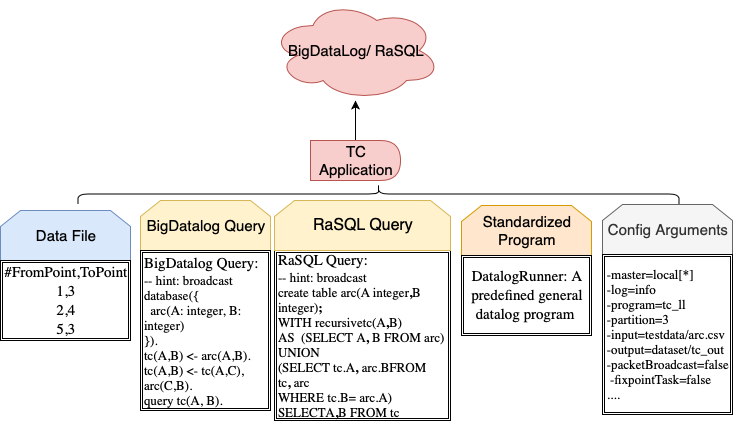
\includegraphics[width=1\linewidth]{Graph/llib/datalogPipeline.png}
		\caption{\small (a) The composition of TC application on custom Datalog platforms. } 
	\end{subfigure}%
	%   \hspace{1em}
	\vspace{\floatsep}
	
	
	\begin{subfigure}{0.6\textwidth}
		\centering
		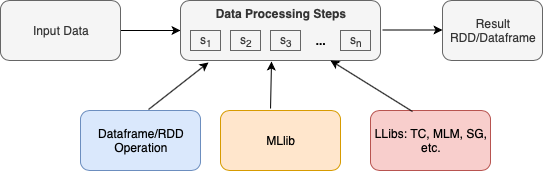
\includegraphics[width=1\linewidth]{Graph/llib/DatalogLib-4.png}
		\caption{\small(b) LLib paradigm} 
	\end{subfigure}%
	\caption{Working paradigm comparison between custom distributed Spark-Based Datalog platforms and the LLib.}\label{fig:comparison}
\end{figure}


\subsubsection{Working session and acquiring data}
\label{sec:data}
In LLib, the first step is to construct a working environment for the Datalog queries and libraries. We respect the customs of building Spark Session and exploit the similar way as following (with Transitive Closure, i.e. TC as a running example):


\vspace{0.5em}
\ex{1.1} - Transitive closure with LLIb:  Working session.
\bldl
session = LLibSession.builder(
).appName(``TC").master(``local[*]"
).getOrCreate()\\

schema = StructType(List(StructField(``Point1", IntegerType, true),\\
StructField(``Point2", IntegerType, true)))\\

df = session.read.format(``csv").option(``header",``false").schema(schema)
.load(``arc.csv")
\eldl
The \textit{LLibSession} synthesizes the  Spark environment and the special designs for logical programming. Within the same session, users are free to utilize the existing Spark libraries like MLlib  or Datalog libraries i.e. LLib. As shown in the third line, the source data can be loaded via the loading function in Spark to a DataFrame \textit{df}. 

\subsubsection{Initializing an executable object of LLib and  mapping the schema}
\textbf{Initialization: }In LLib, the pipeline of the data processing for a typical application is compressed to an object, which you can initialize and set parameters on to process  your data. In this example, we initialize a transitive closure object tc with the TC library, which is pre-defined and included in the LLib. 
Then, we can set the property by built-in functions. 

\vspace{0.5em}
\ex{1.2} - Transitive closure with LLIb:  Initializing TC.
\cldl
import\ edu.ucla.cs.wis.bigdatalog.spark.LLib.TC \\
val\ tc = new\ TC() \\

tc.setDirection(FromCol = "Node1", ToCol = "Node2")
\eldl

\textbf{Schema Mapping: }Among the built-in functions,  all the libraries are required to contain one function called setDirection for schema mapping. This is necessary because we want a more general design that can accept   DataFrame with various schemas as the input.  DataFrame may call an attribute with an arbitrary name but we need to know the corresponding relationship between its attributes and the attribute names mentioned in our library's rules. The Query 2 is a set of Datalog rules for the transitive closure. We have two attributes  From and To in the arc table in the computing logic. The two attributes can be called differently like (Node1, Node2) as shown in the df initialized in Example 1.1. The mapping between (From, To) and (Node1, Node2) can be provided by the setDirection function as shown in the third line of Example 1.2 setDirection (FromCol = "Node1", ToCol = "Node2"). If there is a long mapping list, we can easily extend the current design by  storing the mapping information within a hash table as the transferred parameter to the function.

\vspace{0.5em}
\qr{2} - Transitive closure.
\bldl
database({
	arc(From: integer, To: integer)
}).\\


tc(From,To) \leftarrow arc(From,To).\\
tc(From,To) \leftarrow tc(From,Tmp), arc(Tmp,To). \\
query\ tc(From, To).
\eldl

While processing the data with our library, we need the mapping information. But after processing, the output data's format should be consistent. There is one mechanism to rollback the schema. At the beginning of data processing, we store the schema of input data. Then, in the end, we could use the pre-stored schema to recover. 

When the amount of required attributes by the library matches the amount of columns in the input DataFrame, we could  make full use of the dataset. However, when the dataset contains more attributes than the required, it should be firstly pruned before analysis. As for the condition that the required attributes not included or the dataset contains fewer attributes than  the required, the exception will be raised.



\subsubsection{Execution and persistence}
With the executable object and imported data, the execution and persistence can be merely a one-line calling of a pre-defined function (run, genDF or genRDD) in LLib. These three functions can support the basic requirements to operate data, store the result to a variable or a file. 

\vspace{0.5em}
\ex{1.3} - Transitive closure with LLIb:  Execution and persistence.
\bldl
tc.run(df, output = "File", session) \\
val\ dfNew = tc.genDF(df, session) \\
val\ rddNew = tc.genRDD(df, session) \\

\eldl

\textbf{Execute and persist:} As shown in Example 1.3, the function $run$ is to run the logical programming and persist the result directly to the target address. In the first line, the tc operates df and store the result to File. 

\textbf{Execute and return a DataFrame/RDD:} If the user would like to keep operating the data, they would prefer to get the output data in a form of DataFrame or resilient distributed dataset (RDD) instead of persistence to files. As shown in the second and third lines of the Example 1.3, the dfNew and rddNew will be the outputs and can be further utilized for the next steps of data processing. 


These three functions are implemented for each library of LLib. They expect the input data (df) and the environment (session) as the parameters.  The session information is also needed because during execution, we want the program running within an environment with capability to support the logical 
programming. 


\subsubsection{Operate on multiple datasets}
\label{sec:multiple}
The previous showed TC example operates on only one relation, however there are many applications requiring more than one relation, which causes some changes to the  pipeline. We illustrate the Multi level Market (MLM) Bonus as a typical Datalog application \citep{mlm} acquiring more than one datasets. The application is to calculate the bonus for members of a hierarchical structural Multi Level Marketing  organization. In the organization, the new members are recruited by  and get products from the old members (sponsors). One member's bonus is based on his own sales and a ratio of the sales from the people directly or indirectly recruited by him. The scale of the ratio is a pre-defined rate. 

There are two relations in the MLM Bonus, including the \textit{sponsor} and \textit{sales}. The sponsor relation describes the recruiting relationship among the members, while the sales relation records the profits for each member. In the Datalog rules, the base case is to calculate the member's bonus by the sales table. And the recursive rule is to calculate the bonus based on the basic profits and the profits derived from the downline members.

With the help of LLib, users could implement the MLM Bonus by a pre-defined MLM class in LLib  ignoring the complex logic. The program can be as easy as the follows.

\vspace{0.5em}
\ex{2} -LLib with more than one input relation: Multi level Market Bonus.
\bldl
val\ MLM = new\ MLM() \\
MLM.setDirection(MCol = "M", ProfitCol = "P")\\
MLM.setSecDirection(MCol = "M1", M2Col = "M2") \\
MLM.run(Array(dfSales, dfSponsor), output = "resMLM", session) \\

\eldl
Suppose we already have the two relations stored in dfSales and dfSponsor. In the first line, we build an executable object of MLM. Then, we set the schema mappings for two relations in the next two lines. To operate the data and persist to resMLM file, we use the forth line calling the run function.  The run function of TC application only expects one relation as the input. While dealing with multiple relations, we aggregate the relations in an array as the input. The schema mapping is implemented by adding a new function for the second relation. However, it is possible to  maintain the schema mapping for each relation in a hash function ($h_r$) and use another hash function with the relation's name as the key and the schema mapping information (the hash function, $h_r$) as the value. 
% to store the mapping between the relation and the schema mapping hashing. 
\subsection{LLib Categories}
The supported common Datalog algorithms and utilities in LLib can be  categorized into five groups. We briefly introduce each group and the typical algorithms. 

\textbf{Graph algorithms:} The most common cases of recursive computations  belong to the graph algorithms. In LLib, the typical graph algorithms are Single Source Shortest Path (SSSP), Transitive Closure (TC), Connected Components (CC), and Count Paths (CP). The SSSP  computes the shortest paths from a specific source vertex to all other nodes in a graph with weighted edges. The length of paths are computed iteratively and there is a min aggregation to choose the shortest one. The usage of the SSSP from LLib is as follows.

\vspace{0.5em}
\ex{3} - A graph algorithm (SSSP) supported by LLIb.
\bldl
val\ SSSP = new\ SSSP() \\
SSSP.setFromVertex(vertexID = 1) \\
SSSP.setDirection(fromCol = "From", toCol = "To", costCol = "Cost") \\
SSSP.run(df, output = "resSSSP", session) \\

\eldl
The program differs from the TC example on the second line, where the source vertex is set. The remaining part of the program is identical to TC, which has been fully explained previously. 

CC is to identify the connected components of a graph by attaching and updating each node with a group ID in iterations. The group ID is set each time as the minimum node ID among the nearby nodes. The nodes in a connected component will finally share the same group ID and we just need to compute the number of distinct group IDs. In CP algorithm, we obtain the number of paths from one node to  the other nodes in a graph. The reachability  is transferred iteratively along the edges of graph. The development with CC and CP library will be similar to the TC library, where only the schema mapping is required before execution. 

\textbf{Machine learning algorithms:}
Another series of algorithms, which can be expressed by Datalog queries, are  machine learning algorithms.  Previously, the development for a simple algorithm like Linear Regression or Logistic Regression needs the intensive understanding of the Datalog. With inspirations from Spark MLlib, we provide a more declarative way to develop the machine learning algorithms (including logistic regression, linear regression, SVM, etc.)  on the Datalog platform. 
% We have shown the ML algorithms can be expressed with Datalog, but to attract a wider audience of the data science, it is important to provide a more elegant and succinct way like Spark MLlib. We provide a high-level API for the common ML algorithms including linear regression, logistic regression, etc. 
To illustrate the development with our API, we show a running example exploiting the logistic regression class.

\vspace{0.5em}
\ex{4} - Developing machine learning algorithms with LLib.
\vspace{-2em}
\bldl
//\ Import\ data. 
\\
var\ Vschema = StructType(List(StructField("Id", IntegerType, true), \\StructField(
"C", IntegerType, true),
StructField("V", DoubleType, true),\\ StructField("Y", IntegerType, true))) \\

var\ df = spark.read.format("csv").option("header", "false").schema(Vschema).load("dataV") \\
\\
//\ Training\ on\ the\ input\ relation\ df. \\
import\ edu.ucla.cs.wis.bigdatalog.spark.LLib.DL\_LogisticRegression \\
val\ lr = new\  DL\_LogisticRegression().setMaxIter(10) \\
val\ lrModel = lr.run(df, session)

\eldl
The running environment of our program is still the LLibSession. Then, we can load a pre-processed training dataset stored in a verticalized view with \textit{Vschema} (Id, F, V, T), where the Id is the identification of each training instance; the F is the feature's ID; the V is the feature's value and the T is the label. The verticalized format is beneficial for sparse training data and the transactions of Datalog rules.   After importing the required training functions for logistic regression, we could build an executable training object, \textit{lr}. The \textit{lr} wraps all the logical rules and some required relations (e.g. parameters with default value 0) of the Datalog implementation for the logistic regression training.  While initializing the lr, users can exploit the built-in functions to set the properties like the limit of  iterations, the intial value of parameters, etc. During training (\textit{run}), the session information of the Datalog environment is also required. 
% After fitting the model to \textit{df} relation, the \textit{transform} could make predictions on the testing instances with the pre-trained model \textit{lrModel}.

For comparison, we leverage the Spark MLlib for the above example. The development will become the following, which looks very similar. The differences are: 1)The  input data (\textit{dataS}) do not need verticalization and the schema is not the \textit{Vschema}; 2) An assembler is leveraged to specify the attributes belonging to the features, while in LLib, the verticalized relation is self-explanatory.; 3) The session information is not required during training, while in LLib, the session should be one input parameter for training.
Even though the differences exist, the expressing with Spark MLlib and LLib are extraordinarily similar and both user-friendly.

\vspace{0.5em}
\ex{5} - Machine learning algorithms training with Spark MLlib.
\bldl
//\ Import\ data. \\
var\ schema = StructType(List(StructField("X1", IntegerType, true), \\StructField(
"X2", IntegerType, true),
StructField("X3", DoubleType, true),\\ StructField("label", IntegerType, true))) \\

var\ df = spark.read.format("csv").option("header", "false").schema(schema).load("dataS") \\
\\
//\ Training\ on\ the\ input\ relation\ df. \\
import\ org.apache.spark.ml.Pipeline \\
import\ org.apache.spark.ml.classification.LogisticRegression \\
import\ org.apache.spark.ml.feature.VectorAssembler
\\
val\ assembler = new\ VectorAssembler()
.setInputCols(Array("X1", "X2", "X3"))\\
.setOutputCol("features") \\
val\ lr = new\  LogisticRegression().setMaxIter(10) \\
val\ pipeline = new\ Pipeline().setStages(Array(assembler, lr)) \\
val\ lrModel = pipeline.fit(df) \\
\\
% \\
% //\ Testing\  with\ pre-trained\ model. \\
%     var\ test = spark.read.format("csv").option("header", "false").schema(schema).load("test") \\
% val\ prediction = lrModel.transform(lrModel, test)

\eldl


% Before loading the data, the relation should have been stored in a verticalized view with schema (Id, C, V, Y) as introduced in Section 3.1. 

\textbf{Temporal database queries:}
LLib also supports the transactions on data related to time. For example, in the Interval Coalesce, the goal is to find the smallest set of intervals to cover the input intervals. In Datalog, users are supposed to exploit one rule to find the start points (\textit{S}) of intervals which are not inside the other intervals and another rule to recursively extend the right side of intervals, whose left side belonging to \textit{S}. However, in the LLib, the development will be as simple as follows with \textit{df} (S and E column represents the start point and end point) as the input intervals and the \textit{session} built by LLibSession.


\vspace{0.5em}
\ex{6} - Temporal database query with LLib.
\bldl
val\ Coalesce = new\ Coalesce() \\
Coalesce.setDirection(startCol = "S", endCol = "E") \\
Coalesce.run(df, output = "res", session)
\eldl

\textbf{Financial   applications:}
Except the MLM Bonus mentioned in Section \ref{sec:multiple}, we also support the other financial applications like Bill of Matreials (BOM) \citep{BOM} and  Management. In BOM, one input relation is \textit{assembling} table recording the assembling relation between one item $i$ (or a part of $i$) and its immediate subparts. Another input is \textit{basic} table recording the time cost to deliver the basic parts. The task can be calculating the days required to get  the $i$ ready. We can obtain the required time for each subpart of $i$ and use the maximum time as the result. The calculating of time for each subpart of $i$ should be  execute recursively. In Management, the input table stores the manager and the employees managed by them, and the task is to calculate the total account of employees directly or indirectly managed by one manager. This also requires recursive execution. In LLib, we provide a class wrapping the execution of the BOM or Management and the usage will be similar to the example introduced in Section \ref{sec:paradigm}.

\textbf{Other applications:}
Some other important and classical recursive query applications are also contained in LLib, like same-generation (SG), which identifies pairs of humans with the same hop distance to a common ancestor.  The working paradigm with them will be similar to the Spark MLlib and same as the examples in Section \ref{sec:paradigm}. Here, we will not make repetitive illustrations.

\subsection{Extension of LLib}
LLib also provides a unified template, \textit{TempLib}, to follow when contributing a new algorithm to the LLib. All existing algorithms are developed based on the TempLib. In the TempLib, the provided non-abstract utility functions (like arguments parsing function) can be easily exploited while developing a new algorithm. The template as well contains some requirements needed to be followed. The implementation should at least include three functions (run, genDF and genRDD) for execution and persistence. With the template, the implementation becomes quite uncomplicated. As long as users have the Datalog rules for the algorithm, they can add their own algorithm by doing some minor changes to the existing codes for algorithms like TC. The changes may include a different schema mapping function, or a new function to set an input parameter for your application like the function to set the starting point in the SSSP. 

\subsection{Collaboration with other applications}
The input and output relations in LLib can be both DataFrames, which makes it possible to add a preprocessing  providing the input DataFrames  or  a subsequent processing which takes the DataFrame generated from LLib. The LLib allows users to exploit the Datalog application as a simple step at any place of their  processing pipelines. In this section, we illustrate a concrete example showing the collaborations between LLib and other applications like Spark MLlib or Spark DataFrame Operations. The showed LLib application is the BOM application mentioned previously, and we want to use the linear regression library from MLlib to get the relation between the assembling days and the price of one part. To save the space, we do not show the process to build the session (LLibSession), and load three input relations (dfAssbl, dfBasic, partPrice).  The dfAssbl and dfBasic are two relations in the BOM application storing the assembling relations among parts and the delivery time for basic parts. The partPrice stores the price for each part. With Delivery class from LLib, we could get the \textit{dfRes} storing the cost time for each part. Joining the result relation with the partPrice on the part column will generate a new relation with columns of the day and price. The Linear Regression function from MLlib could train on the result DataFrame. In this example, we can find the  LLib is able to collaborate fluently with other operations in Spark like MLlib (LinearRegression), DataFrame Operations (join).

\vspace{0.5em}
\ex{7} - Collaboration between LLib with other Spark libraries.
\bldl
dfAssbl = dfAssbl.where("Sub < 7")\\
val\ Delivery = new\ Delivery()\\
Delivery.setDirection(PartCol = "Part", SubCol = "Sub")\\
Delivery.setSecDirection(PartCol = "Part", DaysCol = "Days")\\
val\ dfRes = Delivery.genDF(Array(dfAssbl, dfBasic), session)\\
val\ dfRes = dfRes.join(pricePart)\\ 
val\ parsedData = dfRes.rdd.map(row=>\\ LabeledPoint(
row.getAs[Int]("Days"),
Vectors.dense((row.getAs[Int]("Price")))
))\\
val\ numIterations = 10 \\
val\ stepSize = 0.00000001 \\

val\ model = LinearRegressionWithSGD.train(
parsedData,
numIterations,
stepSize)\\

model.save(session.sparkContext, "scalaLinearRegressionWithSGDModel")\\


\eldl



\subsection{Multiple Datalog applications}
A Datalog application can not only work with other Spark libraries but also work with other Datalog applications. The working paradigms of multiple Datalog applications can be in sequential or orthogonal ordering. When they work in sequence, one Datalog application will take another one's result dataset as the input. If they work in an orthogonal ordering, one application's input will be irrelevant with the data processed in other Datalog applications. Both the working paradigms can work with the LLib library, as the library operate on the DataFrame and it is simple to transfer data among applications. This cannot be achieved with the previous Datalog platforms, for they take each Datlog application as a single job to execute, which can hardly collaborate. 

\subsection{User Defined Datalog Function}
Although we have provided all the common Datalog functions in our mind, users may also want to define their own function so that they can use it for futural development. To serve the user-defined datalog function (UDDF), we provide two general classes SingleTableUDDF and MultipleTablesUDDF, which wrap the necessary components to execute the Datalog queries and persist the results to files or a new DataFrame.  The SingleTable is exploited when the UDDF has one input relation while the MultipleTables is exploited when the UUDF has more than one input relations. While utilizing the two classes to specify new Datalog applications, the only required information include Datalog rules and the schema of the basic table (or input table).  

We will show the UDDF with a running example as follows. In the Example 8, we suppose user want to define their SG and Delivery application.   Suppose the \textit{df} stores the  parent-children relations among people. The \textit{dfAssbl}, \textit{dfBasic} stores the assembling relation among parts and the cost days to deliver the basic parts.  The session is a LLibSession. The process to create the df, dfAssbl, dfBasic and session is omitted. For the UDDF of SG, we build an executable object by the SinlgeTableUDDF class and specify the input relation's schema by registerDatalogTable function. The rules are  provided afterwards, which contain the input relation. During execution, the input table (df) and the  query to trigger the  table persistence should be provided. Similarly, for the Delivery, expecting dfAssbl and dfBasic as the input datasets, users are required to build an executable object and register two relations separated by the comma signal. The exeuction can be trigger once the rules and final query are provided. The two executable object (UDDFSG, UDDFDelivery)  are reusable for the future development. If necessary,  users can  build as many UDDFs as they want in a single program.


\vspace{0.5em}
\ex{8} - User-defined Datalog functions.
\bldl
//\ Datalog\ application\ with\ one\ table. \\
val\ UDDFSG = new\ SingleTableUDDF() \\
UDDFSG.registerDatalogTable("rel(Parent: integer, Child: integer)") \\
UDDFSG.rule("sg(X,Y) \leftarrow rel(Parent,X), rel(Parent,Y), X ~= Y. sg(X,Y) \leftarrow rel(A,X),\\ sg(A,B), rel(B,Y).") \\
UDDFSG.run(sourceDataFrame = df, output = "UDDFSG", session, query = "sg(X, Y).") \\
\\

//\ Datalog\ application\ with\ multiple\ tables. \\
val\ UDDFDelivery = new\ MultipleTablesUDDF() \\
UDDFDelivery.registerDatalogTables("  assbl(Part: integer, Sub: integer),\\ basic(Part: integer, Days: integer)")\\
UDDFDelivery.rule("actualdays(Part, mmax<Days>) \leftarrow basic(Part, Days).\\ actualdays(Part, mmax<Days>) \leftarrow assbl(Part, Sub), actualdays(Sub, Days).")\\
UDDFDelivery.run( Array(dfAssbl, dfBasic), output = "UDDFDelivery", session,  \\query = "actualdays(P, D).")




\eldl



\section{LFrame}
\label{lframe}
DataFrame, a widely used data structure, is always supported in different data analytic facilities like Spark SQL, R, Python, but not in Datalog platforms. In this section, we provide a data structure LFrame, wrapping both the Datalog transactions and the common DataFrame transactions. The rest is organized as follows: Section \ref{sec:utility} describes how to convert a normal DataFrame variable to the LFrame variable. Section  \ref{sec:unary} discusses unary operations that operate on one LFrame, while the Section \ref{sec:nary} discusses the N-ary operations using with more than one  LFrame. In each of the Section \ref{sec:unary} and Section  \ref{sec:nary}, we describe one concrete example to illustrate the development with LFrame.

% In Section \ref{sec:expLFrame}, we describe two concrete examples to illustrate the development with LFrame.


\subsection{Conversion from DataFrame to LFrame}
\label{sec:utility}
% Single Frame, Different Frames
To build an LFrame variable, we show the process by the following example.
The entry point of the application using LFrame is the LLibSession, same as the one in LLib, which makes it possible to use both LLib and LFrame within one execution environment. 
The session can  load the data to a DataFrame variable df, but the df cannot execute any logical transaction. To construct an LFrame variable with the  df, a built-in function wrapperDF in LLibSession can be utilized with the session and df as the inputs. 
The session is transferred to provide the Datalog running environment and the df is to supply the dataset with schema.  
The constructed LFrame variable, lframe, could support various Datalog operations like specifying the rules, input tables, persisting the result to a file, etc. These operations are categorised to unary operations and $N$-ary operations and introduced later.

\vspace{0.5em}
\ex{9.1} - Development with LFrame:  Conversion from DataFrame to LFrame.
\bldl
val\ session = LLibSession.builder().appName("LFrame").master("local[*]").getOrCreate() \\
var\ schema = StructType(List(StructField("Parent", IntegerType, true),\\ \ StructField("Child", IntegerType, true)))\\
var\ df = session.read.format("csv").option("header", "false").schema(schema).load("sg")\\
var\ lframe = LLibSession.wrapperDF(df, session)
\eldl

\subsection{LFrame: Unary Operation}
\label{sec:unary}
The unary operation only involves one LFrame object each time. With the lframe in Sec. \ref{sec:utility}, we implement the SG application as following to show the typical provided unary operations. 


\vspace{0.5em}
\ex{9.2} - Development with LFrame:  Unary operations with SG application.
\setcounter{myrow}{0}
\\

$\begin{array}{>{\stepcounter   {myrow} \themyrow : \quad}lrl}
//\ Datalog\ operations\ for \ SG\ application. \\
lframe = lframe.registerCurLFrame("lframe1(Parent: integer, Chile: integer)")\\
lframe = lframe.rules("sg(X,Y) \leftarrow lframe1(Parent,X), lframe1(Parent,Y), X ~= Y")\\
lframe = lframe.rules("sg(X,Y) \leftarrow rel(A,X), sg(A,B), rel(B,Y)")\\
lframe = lframe.rules("sg(X,Y) \leftarrow sg(X,Y)")\\
lframe = lframe.delRule(3)\\
lframe = lframe.query("sg(X,Y)")\\
\\
//\ Execution\ and\ persistence. \\
lframe.run(output = "SG")\\
val\ dfRes = lframe.genDF()\\
val\ rddRes = lframe.genRDD()
\\ \\
//\ Normal\ DataFrame\ operations. \\
lframe.nonRecursive().where("X < 10").select("X").collect().foreach(println) \\
\end{array}$
\\

There are six categories of unary operations included in the above example. 
\begin{itemize}
	\item \textbf{Registering one LFrame as a base relation.} In the line 2, the registerCurLFrame is to register the lframe as a base relation so that the Datalog rules can utilize it as a given dataset. While registering, users are free to rename the dataset's columns and the LFrame will map the columns according to the order of appearance. 
	\item \textbf{Appending rules.} The main body (line~3 to~5) of a Datalog program is a finite set of rules. To state the rules, the function called "rules" can be exploited. Whenever the function is utilized,  a new rule will be appended to the existing rule sets owned by the lframe.
	\item \textbf{Removing rules.} If one rule is wrongly appended, it can be removed by the delRule (line 6) function using its index. The provided index variable can be also an array, which removes more than one rule.
	\item \textbf{Specifying output relation.} To evaluate the application, the query function (line 7)  assists to point out the output relation, which is the sg relation in the SG application. The generated result LFrame will store the output dataset in the schema specified in query, (X, Y).  
	\item \textbf{Execution and persistence.} In DataFrame, the evaluations are lazy. Similarly, the LFrame's evaluation is lazy until the run action is triggered.  As shown in the second part of the code (line~9 to~12), the run function will store the result relation to a file and if a user want to restore the result to a DataFrame or RDD, the genDF or genRDD function can be considered. 
	\item \textbf{Non-recursive transactions.} The design of LFrame is to wrap both the Datalog transactions and the normal DataFrame transactions. When a normal DataFrame transaction is required, like the line 15 shows, the nonRecusive function will convert the execution to the normal DataFrame execution and accept all the DataFrame operators afterwards. 
\end{itemize}
Compare the LFrame with DataFrame, we can find they work in  analogous ways  but LFrame can support more operations. A more compact way to express the transactions from line 2 to 7 is to list them back to the lframe one by one like the line 15. 
\subsection{LFrame: N-ary Operation}
\label{sec:nary}
In the previous SG example, only one relation is contained in the Datalog application, while in this section, we illustrate the transaction (registerMoreDFs)  embroiling more relations like the join operator of the relational database or DataFrame. We adopt the Delivery Datalog application as a running example, for it contains both the assembly and the basic relations. The assembly relation stores assembling relation among parts and the delivery days of basic parts are stored in the basic relation. The expected output should be the  time spent for each part.

\vspace{0.5em}
\ex{9.3} - Development with LFrame:  $N$-ary operations with Delivery application.
\setcounter{myrow}{0}
\\

$\begin{array}{>{\stepcounter   {myrow} \themyrow : \quad}lrl}
var\ schemaAssbl = StructType(List(StructField("Part", IntegerType, true),\\ \quad StructField("Sub", IntegerType, true)))\\
var\ dfAssbl = session.read.format("csv").option("header", "false").\\ \quad schema(schemaAssbl).load("assbl")\\
var\ schemaBasic = StructType(List(StructField("Part", IntegerType, true),\\ \quad StructField("Days", IntegerType, true)))\\
var\ dfBasic = session.read.format("csv").\\ \quad option("header", "false").schema(schemaBasic).load("basic.csv")\\
\\
//\ Datalog\ operations\ for \ Delivery\ application. \\
var\ lfAssembly = DatalogLibSession.wrapperDF(dfAssbl, session) \\
lfAssembly = lfAssembly.registerCurDF("assbl(Part: integer, Sub: integer)")\\
lfAssembly = lfAssembly.\textbf{registerMoreDFs}(otherDF = Array(dfBasic), \\ \quad registers = Array("basic(Part: integer, Days: integer)"))  \\
lfAssembly = lfAssembly.rules("actualdays(Part, mmax<Days>) \\ \quad \leftarrow basic(Part, Days)") \\
lfAssembly = lfAssembly.rules("actualdays(Part, mmax<Days>) \\ \quad \leftarrow assbl(Part, Sub), actualdays(Sub, Days)")\\
lfAssembly = lfAssembly.query("actualdays(P, D)")\\
lfAssembly.run(output = "Delivery_1")\\


\end{array}$
\\

In the example, we do not show the process of establishing the execution environment (session) to save space. We firstly load two relations to DataFrame objects dfAssbl and dfBasic (line~1 to~8). Then, the dfAssbl is converted to an LFrame variable with Datalog functions encapsulated. To exploit the relation as the base relation, the registerCurDF function is exploited in line 12. 

The above mentioned steps solely rely on one relation, however, the basic relation is required in the Delivery application. To involve more datasets, the registerMoreDFs function (line~13) need to be utilized. The input parameters include an array of DataFrames to be registered and another array of schemas exploited to register them. The two arrays are ordered and have one-to-one correspondence. Thereupon, the rules can take these DataFrames as the base relations to use. To construct the rule sets, the rules function is adopted multiple times. Eventually, the output relation specified by query function will be stored to the address contained in the run function (line~19 to~20). 

% Binary: 2
% Ternary: 3


% Single Frame, Different Frames


\section{Conclusion}
\label{llib:conclusion}

In this chapter, we have shown the LLib encapsulating typical Datalog algorithms, which follows the data scientists' customs  and requires less logical programming expertise.  For the possible  extensions of LLib, we provide not only a unified template for normalizing the contribution, but also some utilities to simplify the extending process.  With some running examples, we  demonstrate the benefit of designing the LLib as the DataFrame-based API is that the Datalog algorithm can  become a single step within the data processing pipelines collaborating with other Spark operations. For the audience who has more logical programming experience and would like to design their own applications, we also provide an LFrame API containing both logical and DataFrame-based operations. A simple conversion approach between the DataFrame and LFrame is also given for a simplified developing. Moving forward, we have  plenty of new algorithms and logical oeprations to add for the LLib and LFrame separately. We plan to make the LLib and LFrame more general for different languages like Python, R. We also  would like to implement the two interfaces on other distributed platforms or crossing various platforms in a way like a polystore system \citep{duggan2015bigdawg}
